\chapter{Durchführung}\label{cha:durchfuehrung}
\section{Vorbereitung}\label{sec:vorbereitung}
\subsection{Auswahl der Umgebung und Höhe}\label{sub:auswahlUmgebung}
Um das Experiment durchzuführen müssen verschiedene Vorbereitungen vorgenommen werden. Zuerst muss der Ort ausgewählt werden. Um das Experiment möglichst erfolgreich und präzise zu halten, sollte es in einem möglichst dunklen Raum durchgeführt werden. Für diese Arbeit wurde die Dunkelkammer (Zimmer G10) der Kantonsschule am Burggraben zur Verfügung gestellt. Ein weiterer Punkt der Vorbereitung ist der Untergrund, auf dem das Experiment steht. Im Experimentierkasten kommen Verlängerungsstäbe mit, die dazu dienen das Experimentieren angenehmer zu machen. Das Problem mit diesen Stäben ist, dass sie Vibrationen nicht weghalten und das Experiment sehr anfällig für diese ist. In dieser Arbeit wurde die Plattform auf ein Holzklotz gelegt, damit das Experiment auf Augenhöhe ist bei gestrecktem Rücken. Die Plattform sollte gerade stehen. Das kann man mit der Wasserwaage auf der Plattform kontrollieren. Falls die Plattform schräg sein sollte, kann man mit den veränderbaren Füssen die Plattform ausebenen. Mit diesem Holzklotz hatte das Experiment einen festen Untergrund und war somit bereit für das Einstellen des optischen System. 

\subsection{Kondensatorenabstand messen}\label{sub:kondensatorenabstand}
Der nächste Schritt für die Vorbereitung ist das Messen des Abstandes zwischen den beiden Kondensatoren. Das Wichtige bei diesem Schritt ist, dass die Spannung abgeschaltet ist. Zuerst wird das Gehäuse der Betrachtungskammer abgenommen. Danach wird die obere Platte vorsichtig weggenommen und die darunter liegende Platte aus Kunststoff auch. Im Experimentierkasten befindet sich eine Schieblehre. Damit misst man die Dicke der Kunststoffplatte. Wichtig ist, dass man am inneren Rand der Platte misst und nicht am äusseren, da der äussere Rand ein Bisschen dicker ist. Jetzt kann der Wert direkt abgelesen und notiert werden. 

\section{Das optische System ausrichten}\label{sec:optischesSystem}
\subsection{Das Betrachtungsfernrohr fokussieren}
Die Betrachtungskammer sollte jetzt wieder zusammengebaut werden, das Gehäuse aber noch nicht. Auf der Platte soll der Fokussierdraht abgeschraubt werden und Vorsichtig in das Loch in der Mitte der oberen Kondensatorenplatte eingeführt werden. Danach muss die Halogenlampe angeschlossen werden. Dafür muss der Stecker des 12 V DC Transformator an die Lampe angeschlossen werden, dann sollte die Lampe leuchten. Jetzt muss zuerst das Fadenkreuz in Fokus gesetzt werden. Dafür muss man den Fadenkreuz-Fokussierring drehen bis man das komplette Gitter scharf sieht. Dann sollte man den Draht anschauen durch das Betrachtungsfernrohr und den Tröpfchen-Fokussierring solange drehen bis man den Draht scharf sehen kann. 

\subsection{Die Halogenlampe einstellen}\label{sub:Halogenlampe}
Mit dem horizontalen Einstellknopf der Halogenlampe soll das Licht auf der horizontalen Ebene richtig fokussiert werden. Damit das Licht am besten fokussiert ist, muss der rechte Rand des Drahtes am hellsten sein. Das heisst, im grössten Kontrast zur linken Seite des Drahtes stehen. Mit dem vertikalen Einstellungsknopf muss das Licht auf der Mitte des Gitters / Fadenkreuz am besten zu sehen sein. Wenn alles fertig eingerichtet ist, sollte der Fokussierdraht wieder in die Vertiefung in der Platte verschraubt werden.

\section{Funktionen der Steuerung}\label{sec:funktionen}
\subsection{Kondensatorenspannung Schalter}\label{sub:Spannungsschalter}
Dieser Schalter ist ein Spannungswechsler der beiden Kondensatoren. Mit diesem Schalter kann die Richtung des Elektrischen Feld $E$ gewechselt werden. Er besitzt auch drei verschiedene Positionen. Die erste, plates grounded, bedeutet, dass keine der beiden Kondensatoren geladen ist, es wirkt dabei keine Kraft auf die Tröpfchen. Die zweite Position ist TOP PLATE -, das bedeutet, dass die obere Platte negativ geladen ist und somit ein elektrisches Feld nach unten zeigt. Die letzte Position ist TOP PLATE +, das bedeutet, dass die obere Platte positiv geladen ist und somit ein Feld nach oben wirkt. 

\subsection{Der Ionisationsquelle Schalter}\label{sub:ionisationquelle}
Der Schalter für die Ionisation hat 3 verschiedene Positionen. Die An-Position, die Aus-Position und die Tröpfchensprüh-Position. Wenn der Schalter auf der Aus-Position ist, wird die Ionisationsquelle komplett abgeschirmt und es können keine Alphateilchen in die Kammer gestrahlt werden. Bei der An-Position ist dieser Schirm nicht mehr da und die Öltröpchen können angestrahlt werden. Die dritte Position, die Tröpfchensprüh-Position, muss geschaltet werden, wenn die Ölrtöpchen eingesprüht werden. Bei dieser Position öffnet sich ein kleines Loch in der Kammer, damit die Luft ausströmen kann, wenn das Öl eingesprüht wird.

\begin{figure}[ht]
	\begin{center}
		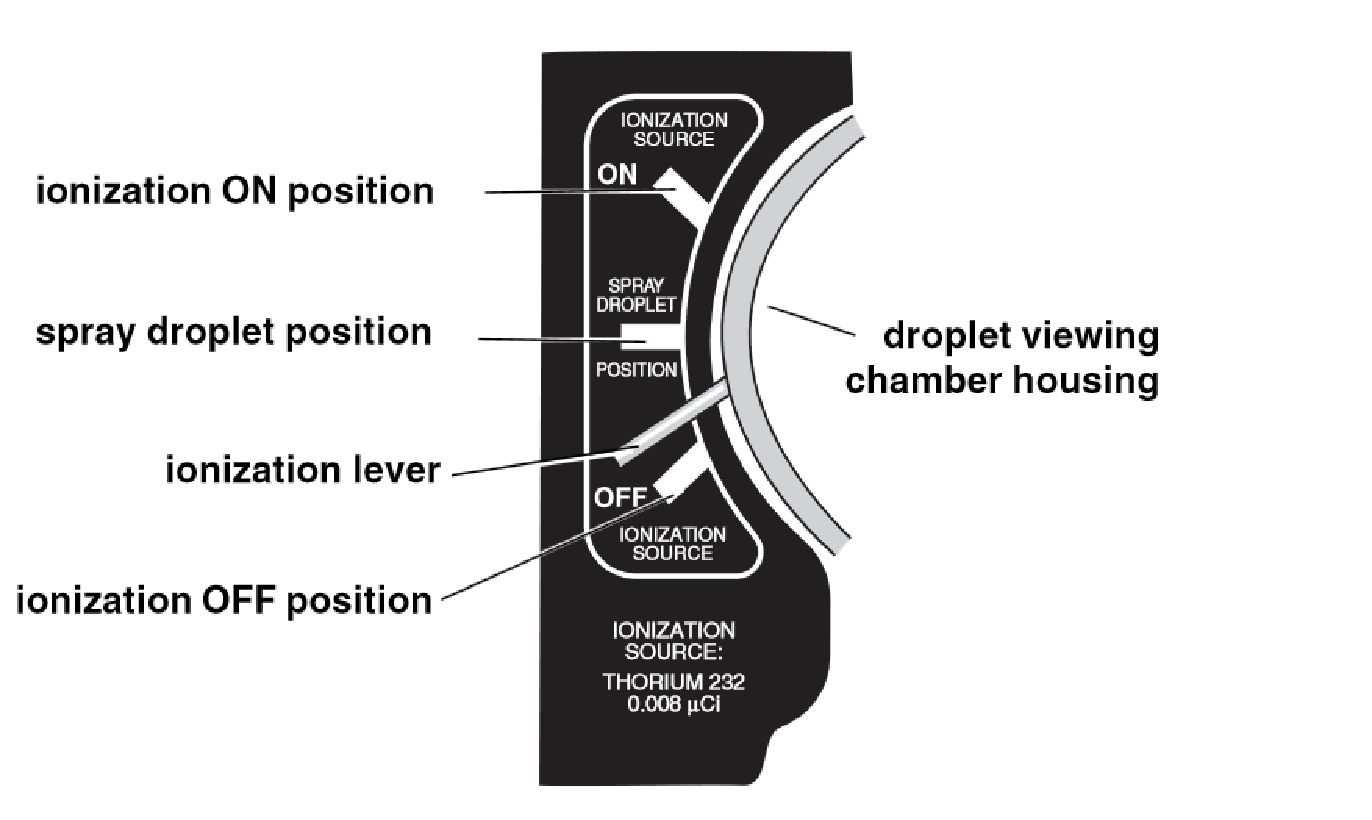
\includegraphics[scale=0.5]{bilder/pdf/Schalterfunktionen.pdf}
		\caption{Schalterpositionen der Ionisationsquelle}
		\label{fig:Schalterpositionen}
	\end{center}
\end{figure}

\section{Messen und Einstellen der Spannung}\label{sec:spannung}
Zuerst muss die Gleichstromquelle an die Plattform, über die farbigen Anschlüsse, angeschlossen werden. Das digitale Multimeter kann direkt bei den Kontakten parallel eingebaut werden. Jetzt muss das Multimeter eingeschaltet werden, dabei muss die Gleichstromspannung ausgewählt werden. Wenn die Stromquelle eingeschaltet wird sollte das Multimeter ungefähr 500V anzeigen. Wenn das nicht der Fall ist muss man die Spannung noch richtig einstellen bei der Stromquelle. Wichtig zu wissen ist, dass man keinen elektrischen Schock kriegen kann von den Kondensatoren, da in diesen grosse Widerstände eingebaut sind, die dies vorbeugen.

\section{Temperatur in der Tröpfchenkammer}\label{sec:Temperatur}
Die letzte Einstellung, die gemacht werden muss, um danach mit dem eigentlichen Experimentieren zu beginnen, ist die Temperatur zu messen innerhalb der Tröpfchenkammer. Die Temperatur braucht man, um die Zähigkeit der Luft herauszufinden. Da man die genaue Temperatur nicht mit einem Thermometer herausfinden kann, kann man über die Beziehung vom elektrischen Widerstand in den Kondensatoren gehen. Den Widerstand wird gleich wie die Spannung gemessen. Auf der Platte hat es Anschlüsse für ein digitales Multimeter, das sollte auf elektrischer Widerstand eingeschaltet werden. Dieser proportionale Zusammenhang kann man auf der Tabelle ablesen. Wichtig ist, dass die Stromquelle nie an die Anschlüsse für den Widerstand angeschlossen werden, weil so das Experiment kaputt gehen könnte. Der Widerstand sollte ungefähr bei 1 - 4 Megaohm sein.

\begin{figure}[ht]
	\begin{center}
		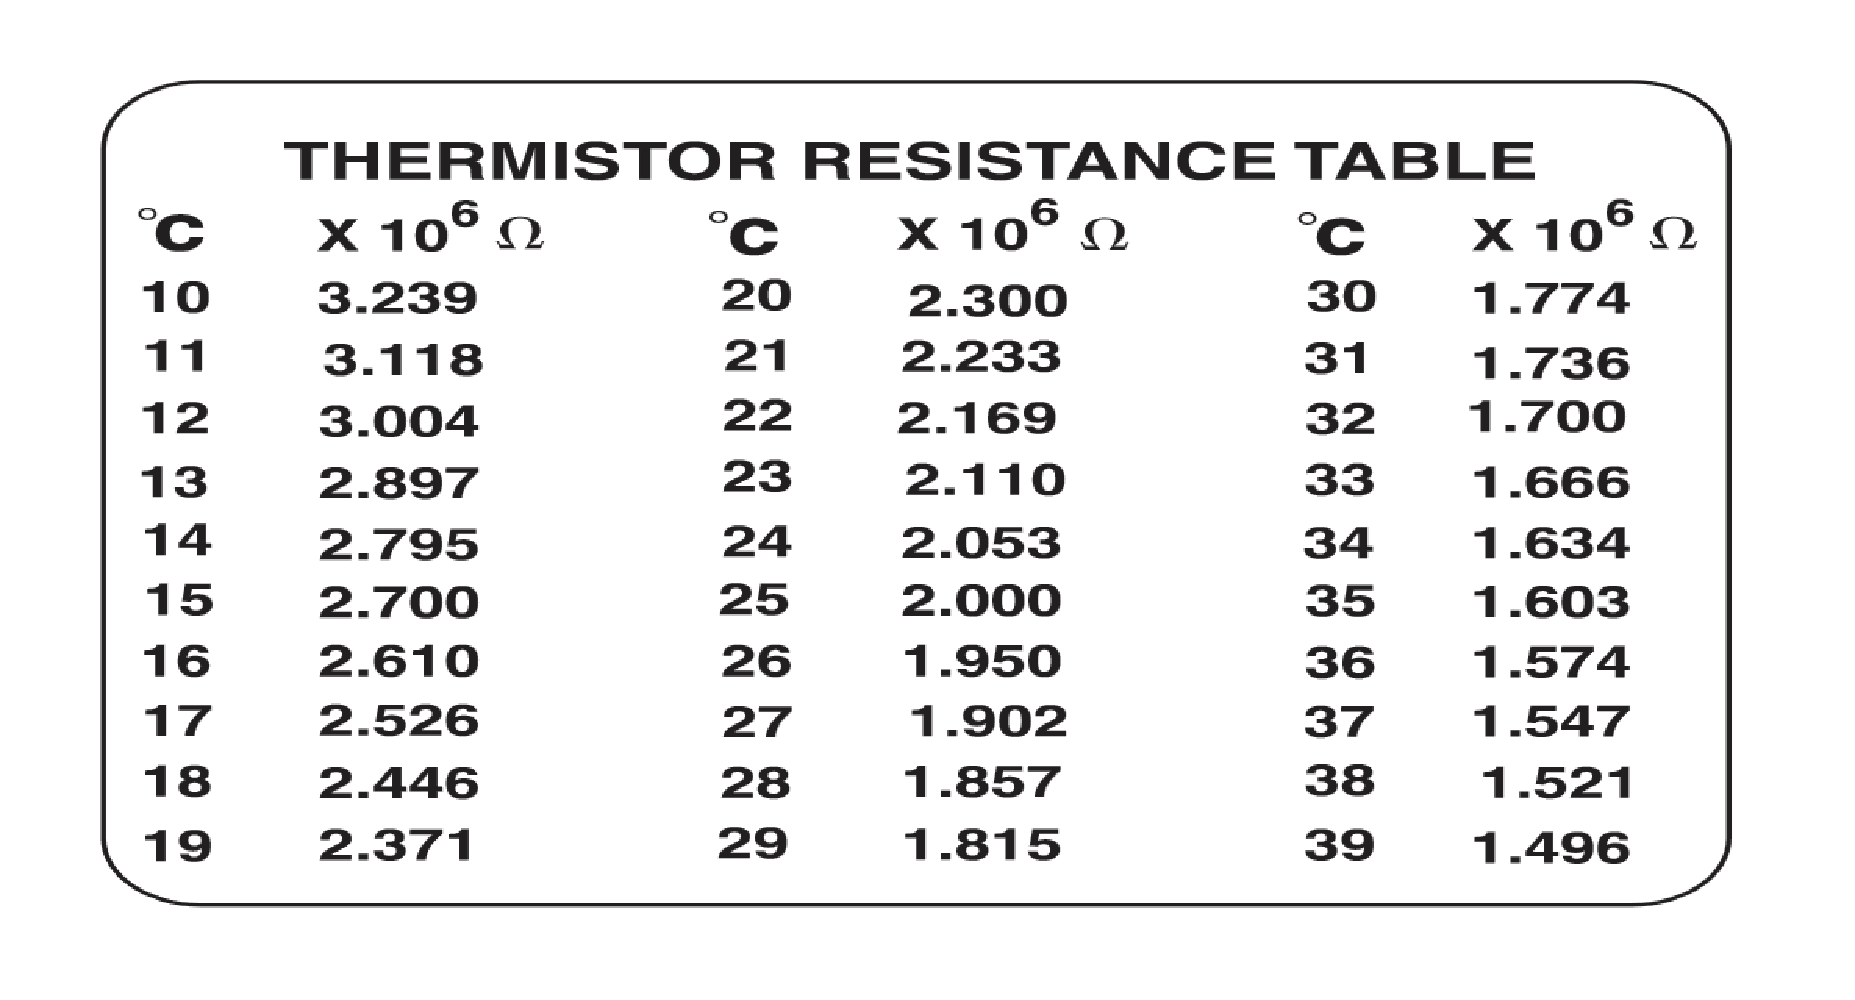
\includegraphics[scale=0.25]{bilder/pdf/TemperaturTabelle.pdf}
		\caption{Abhängigkeit von Temperatur und elektrischer Widerstand}
		\label{fig:widerstandTemperatur}
	\end{center}
\end{figure}

\section{Das Experimentieren}\label{sec:durchfuehrung}
Bevor man beginnt, muss die ganze Kammer wieder zusammengebaut werden und der Tröpfchenlochschutz sollte auf die Einsparung der oberen Platte gesetzt werden. Dieser Schutz verhindert, dass während dem Experimentieren weitere Tröpfchen in die Betrachtungskammer gelangen. Jetzt misst man nochmals kurz die Spannung und Temperatur, um dann mit dem Experimentieren zu starten.

\subsection{Tröpfchen Einsprühen}\label{sub:tröpfchensprühen}
Der Erste Schritt ist das Vorbereiten des Ölsprühers. Dazu gibt man Mineral Öl, bei welchem die Dichte bekannt ist (z.B. das zugehörige Squibb \#5597 Mineral Oil mit Dichte: $886 kg/m^3$), in den Zerstäuber. Jetzt versucht man Tröpfchen zu erzeugen mit dem Zerstäuber. Für das sollte schnell nacheinander fest auf das Kissen gedrückt werden, bis auf einem Papier kleine Tröpfchen zu sehen sind.
\begin{figure}[h]
	\begin{minipage}[t]{0.45\textwidth}
		\centering
		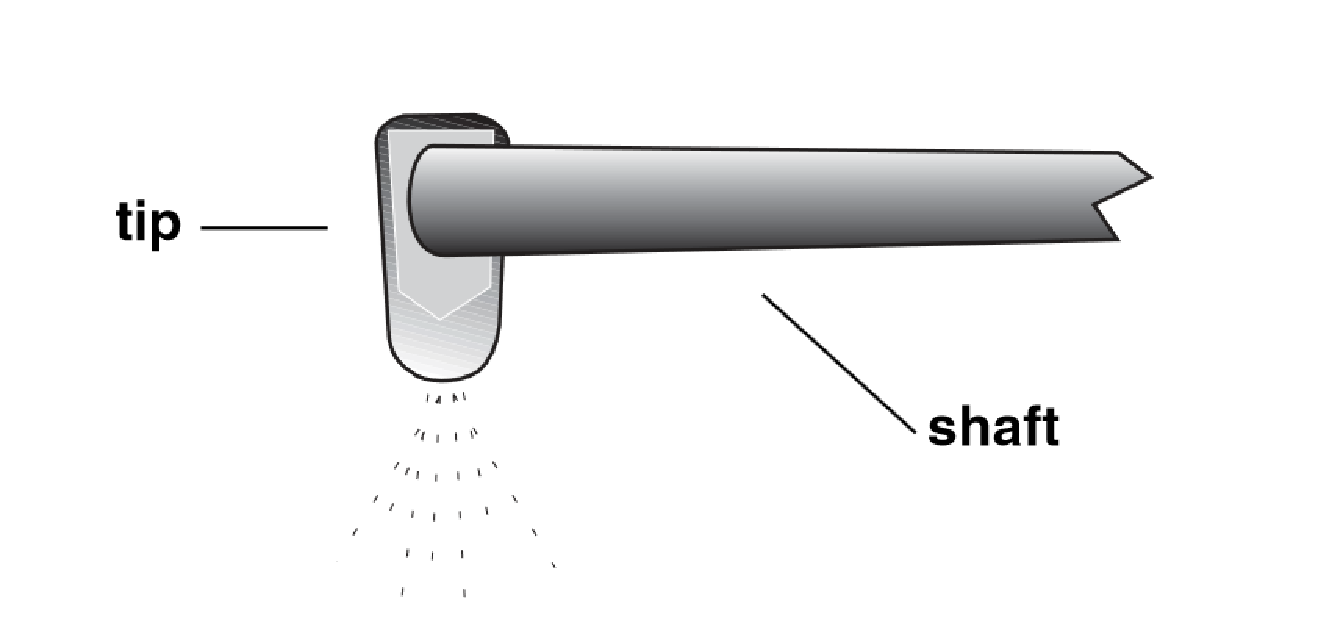
\includegraphics[width=\textwidth]{bilder/pdf/zerstauberSpitze.pdf}
		\caption{Korrekte Position von Spitze zur Achse}
		\label{fig:zerstauberSpitze}
	\end{minipage}
	\hfill
	\begin{minipage}[t]{0.45\textwidth}
		Die Spitze des Zerstäubers muss nach unten schauen. Genau 90° zur Achse. (siehe \autoref{fig:zerstauberSpitze})
	\end{minipage} 
\end{figure}

Nach diesem Schritt sollte der Schalter der Ionisationsquelle auf Tröpfchensprüh-Position gebracht werden, damit Luft während dem Einsprühen aus der Kammer entfliehen kann. Da die Spitze des Zerstäubers genau nach unten zeigt kann sie jetzt direkt in das vorgesehene Loch auf dem Deckel des Gehäuses angebracht werden. Jetzt muss durch das Betrachtungsfernrohr geschaut werden und gleichzeitig einmal kräftig auf das Kissen des Zerstäubers drücken. Jetzt mit kleineren schwächeren Stössen auf das Kissen die Tröpfchen ins Sichtfeld des Betrachters bringen. Wenn man einen grossen Haufen mit kleinen goldenen Punkten sieht, muss der Schalter auf die Aus-Position gebracht werden. 

Das Einsprühen von den Tröpfchen ist am Anfang sehr schwierig und wird nicht auf das erste Mal funktionieren. Es gibt nicht die richtige Technik, den Zerstäuber zu bedienen. Der Experimentierer muss seine eigene Technik finden den Zerstäuber zu bedienen. Das kann sehr viel Zeit in Anspruch nehmen. In dieser Arbeit funktionierte es am besten, wenn man einmal fest gedrückt hat und danach kleinere schwächere Stösse gegeben hat.

Falls zu viele Tröpfchen im Sichtfeld des Betrachters sind, sollte man drei bis vier Minuten warten und dann sollten die meisten Tröpfchen verschwunden sein. Man kann dann gemütlicher weiter Experimentieren.

\subsection{Auswahl des richtigen Tröpfchen}\label{sub:auswahlTropfen}
Von den Tröpfchen, die sichtbar sind, sollte eines Ausgewählt werden, dass ungefähr $0.02 - 0.05 mm/s$ fällt wenn der Schalter der Kondensatoren auf plates grounded steht und sich mit dem Schalter nach oben und unten bewegen lässt. Diese Beschreibung ist sehr schwierig zu messen. Einen Tipp, ein Tröpfchen das ungefähr 15 Sekunden braucht für die Distanz zwischen zwei Hauptlinien auf dem Gitter ($0.5mm$), fliegt etwa $0.03 mm/s$. 

Falls immernoch zu viele Tröpfchen im Sichtfeld sind kann man auch für ein paar Sekunden die Kondensatoren laden und die meisten Tröpfchen werden wegfliegen. Da sich nicht alle Tropfen bewegen lassen, weil sie eine Nettoladung von 0 C haben, kann man den Ionisationsschalter für drei bis fünf Sekunden auf die An-Position schalten. Danach sollten sich alle Tröpfchen bewegen lassen. \\

Wenn ein Tröpfchen gefunden wurde mit diesen Voraussetzungen kann man es mit dem Fokussierring noch schärfer machen. Das entlastet die Augen und man kann länger beobachten. Der Fokus ist am besten wenn das Tröpfchen wie eine goldene Nadelspitze aussieht.

\subsection{Daten sammeln mit der Fall und Steigzeit}\label{sub:datenFallundSteig}
Um die Ladung eines Tröpfchens zu bestimmen, muss die Steiggeschwindigkeit (Kondensatoren geladen) und die Sinkgeschwindigkeit (Kondensatoren nicht geladen) gemessen werden. Die genauste Messung ergibt sich wenn man die Zeit stoppt vom erste grosse Linie Überschreiten bis zum Überschreiten der zweiten grossen Linie. Diese Linien sind genau 0.5 mm voneinander entfernt. Wenn man die Zeit hat, die das Tröpfchen für diese Distanz gebraucht hat, kann man die Geschwindigkeit $v$ berechnen mit der einfachen Formel $v = \frac{s}{t}$. Ein Beispiel, wenn ein Tröpfchen genau 15 Sekunden für die Strecke gebraucht hat rechnet man: $v = \frac{s}{t} = \frac{0.5mm}{15s} = 0.033 mm/s = 3.3 \cdot 10^{-5} m/s$. 

Für ein genaues Ergebnis sollte man die Geschwindigkeiten ungefähr 5 - 15 mal von einem Tropfen messen. \\

Nach der ersten Messung sollte provisorisch die Ladung des Tropfes gemessen werden. Falls die Ladung mehr als fünf mal die Elementarladung beträgt, sollte man für die nächsten Messungen langsamere Tröpfchen wählen. 

Jetzt sollten neue Tröpfchen eingesprüht werden und die Geschwindigkeiten erneut gemessen werden bis das Tröpfchen spontan seine Ladung ändert oder aus dem Sichtfeld verschwindet. Mit dem Ionisierungsschalter kann die Ladung eines Tröpfchens verändert werden. Jetzt kann man die neuen Geschwindigkeiten messen. Dieser Schritt sollte so oft wie möglich wiederholt werden. Wenn das Auge zu müde wird, kann man die verschiedenen anderen Faktoren wie die Spannung, die Zähigkeit der Luft, die Dichte des Öls und den Luftdruck messen. Alle Messungen sollten schön in einer Tabelle eingetragen werden, danach kann man anfangen die Ladungen jeder Messung zu berechnen.

\subsection{Methode für die Berechnung der Ladung}\label{sub:methodeBerechnung}
Mit der Formel in \autoref{eq:qRadius} kann zuerst der Radius $a$ berechnet werden:
\begin{equation*}
	a \ = \ \sqrt{\left( \frac{b}{2p}\right)^2 + \frac{9\eta v_f}{2\rho g}} - \frac{b}{2p}
\end{equation*}

\noindent Dann kann die Masse $m$ des Tröpfchens berechnet werden indem man die Formel für den Radius in die Formel für die Masse Substituiert:
\begin{equation*}
	\begin{split}
		m & \ = \ \frac{4}{3}\pi a^3 \rho \\
		& \ = \ \frac{4}{3}\pi \left( \sqrt{\left( \frac{b}{2p}\right)^2 + \frac{9\eta v_f}{2\rho g}} - \frac{b}{2p} \right)^3 \rho
	\end{split}
\end{equation*}

\noindent Der letzte Schritt ist die Masse $m$ in der \autoref{eq:hauptgleichung} zu substituieren:
\begin{equation*}
	\begin{split}
		q & \ = \ \frac{m g (v_f + v_r)}{Ev_f} \\
		& \ = \ \frac{4}{3} \pi \rho g \left( \sqrt{\left( \frac{b}{2p}\right)^2 + \frac{9\eta v_f}{2\rho g}} - \frac{b}{2p} \right)^3 \frac{(v_f + v_r)}{Ev_f}
	\end{split}
\end{equation*}

\noindent Wenn man das $E$ jetzt noch mit der \autoref{eq:elektrischeFeldstärke} ersetzt hat man die Ladung $q$ eines Tröpfchens:
\begin{equation*}
	q_{tröpfchen} \ = \ \frac{4}{3} \pi \rho g \left( \sqrt{\left( \frac{b}{2p}\right)^2 + \frac{9\eta v_f}{2\rho g}} - \frac{b}{2p} \right)^3 \frac{d(v_f + v_r)}{Vv_f}
\end{equation*}







